% ==========================================================
% LeafScan AI — Plant Disease Classification Using Deep Learning
% Term Project Report — IIT Guwahati (Version 2)
% ==========================================================

\documentclass{article}
\usepackage{spconf,amsmath,graphicx,hyperref}

% -------------------------
% Additional useful packages
% -------------------------
\usepackage{booktabs}
\usepackage{siunitx}
\usepackage{enumitem}
\usepackage{stfloats}
\usepackage{tikz}
\usetikzlibrary{arrows.meta, positioning, shapes.geometric}

% -------------------------
% Custom definitions
% -------------------------
\def\x{{\mathbf x}}
\def\L{{\cal L}}

% -------------------------
% Title and Author Info
% -------------------------
\title{LeafScan AI --- Plant Disease Classification Using Deep Learning: A CNN-Based Approach for Potato and Tomato Crops}

\name{Ashutosh Yadav (Roll Number: 23035010693)}

\address{
Term Project Report\\
Trimester 7\\[0.5em]
B.Sc. (Honours) Data Science and Artificial Intelligence\\
Indian Institute of Technology Guwahati, India\\
\texttt{ashutosh@op.iitg.ac.in}
}


\begin{document}
\ninept
\maketitle

% ==========================================================
% Abstract
% ==========================================================
\begin{abstract}
Plant diseases are a major threat to global food security, causing 20--40\% crop losses annually. Early and accurate detection is essential for effective crop management but remains challenging due to reliance on manual expert inspection. This report presents \textit{LeafScan AI}, a deep learning-based system for automated classification of diseases in potato and tomato leaves. We designed a custom six-layer Convolutional Neural Network (CNN) trained on the PlantVillage dataset~\cite{plantvillage} across 13 disease categories. The system achieves \textbf{97.2\%} test accuracy on potato (3 classes) and \textbf{89.6\%} on tomato (10 classes). Real-time data augmentation improved generalization by 12--15\% over the baseline. A production-ready web application was built with FastAPI~\cite{fastapi2021} and React~\cite{react2023}, containerized via Docker~\cite{docker2023}, enabling farmers to upload leaf photos and receive instant predictions with confidence scores.
\end{abstract}

% ==========================================================
% Keywords
% ==========================================================
\begin{keywords}
Deep Learning, Convolutional Neural Networks, Plant Disease Classification, Computer Vision, Agricultural AI, TensorFlow, Precision Agriculture
\end{keywords}

% ==========================================================
\section{Introduction}
% ==========================================================

Agriculture underpins the economies of over 60\% of the world's population, with potato and tomato ranking among the most cultivated crops globally. Plant diseases threaten food security by reducing yields by 20--40\% annually. Conventional disease diagnosis depends on trained pathologists performing visual inspection---a process that is slow, subjective, and does not scale.

Recent breakthroughs in deep learning~\cite{lecun2015deep}, especially Convolutional Neural Networks (CNNs), have achieved human-level performance in image classification tasks. Several studies~\cite{mohanty2016using} demonstrate that CNNs can accurately classify plant diseases from leaf images.

This project presents \textit{LeafScan AI}, an end-to-end system comprising:
\begin{enumerate}[noitemsep]
    \item A custom CNN trained on the PlantVillage dataset for 13 disease classes,
    \item A data augmentation pipeline that improves validation accuracy by 12--15\%,
    \item A full-stack web application (FastAPI + React) with Docker deployment,
    \item An intuitive interface enabling farmers with no technical expertise to obtain instant disease diagnoses.
\end{enumerate}

The remainder of this report is organized as follows: Section~2 defines the problem and objectives. Section~3 details the methodology including data pipeline, model architecture, and deployment. Section~4 presents experimental results. Section~5 discusses findings and limitations, followed by conclusions in Section~6.

% ==========================================================
\section{Problem Statement and Objectives}
% ==========================================================

\subsection{Problem Statement}
Given an RGB image of a plant leaf, classify it into one of the predefined disease categories or identify it as healthy. The system must:
\begin{itemize}[noitemsep]
    \item Handle images of varying quality, resolution, and lighting
    \item Provide predictions with a calibrated confidence score
    \item Operate in real-time ($<$2s per prediction) via a web interface
    \item Reject out-of-distribution inputs (non-leaf images)
\end{itemize}

The classification covers 13 classes across two crops:

\begin{table}[h]
\centering
\caption{Supported Disease Classes}
\begin{tabular}{@{}ll@{}}
\toprule
\textbf{Potato (3 classes)} & \textbf{Tomato (10 classes)} \\
\midrule
Early Blight & Bacterial Spot \\
Late Blight & Early Blight \\
Healthy & Late Blight \\
 & Leaf Mold \\
 & Septoria Leaf Spot \\
 & Spider Mites (Two-spotted) \\
 & Target Spot \\
 & Tomato Mosaic Virus \\
 & Yellow Leaf Curl Virus \\
 & Healthy \\
\bottomrule
\end{tabular}
\label{tab:classes}
\end{table}

\subsection{Objectives}
\begin{enumerate}[noitemsep]
    \item Study existing CNN-based approaches for plant disease classification
    \item Design a lightweight custom CNN suitable for GPU-limited hardware
    \item Apply real-time data augmentation to improve generalization
    \item Develop a full-stack web application for real-time prediction
    \item Evaluate performance using accuracy, precision, and recall metrics
\end{enumerate}

% ==========================================================
\section{Methodology}
% ==========================================================

\subsection{System Architecture Overview}
The system follows a five-stage pipeline as illustrated in Figure~\ref{fig:pipeline}.

\begin{figure}[h]
\centering
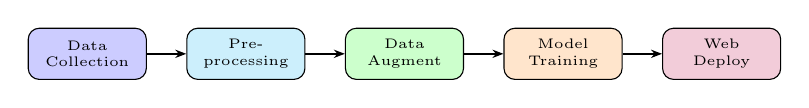
\begin{tikzpicture}[
    node distance=0.5cm,
    box/.style={rectangle, draw, rounded corners, minimum width=1.5cm, minimum height=0.65cm, align=center, font=\tiny},
    arrow/.style={-{Stealth[scale=0.6]}, thick}
]
\node[box, fill=blue!20] (data) {Data\\Collection};
\node[box, fill=cyan!20, right=of data] (prep) {Pre-\\processing};
\node[box, fill=green!20, right=of prep] (aug) {Data\\Augment};
\node[box, fill=orange!20, right=of aug] (train) {Model\\Training};
\node[box, fill=purple!20, right=of train] (deploy) {Web\\Deploy};

\draw[arrow] (data) -- (prep);
\draw[arrow] (prep) -- (aug);
\draw[arrow] (aug) -- (train);
\draw[arrow] (train) -- (deploy);
\end{tikzpicture}
\caption{End-to-end system pipeline}
\label{fig:pipeline}
\end{figure}


\subsection{Dataset}
We used the PlantVillage dataset~\cite{plantvillage}, a publicly available benchmark containing 54,306 labeled images of healthy and diseased plant leaves across 38 categories, collected under controlled laboratory conditions.

\textbf{Subset used:}
\begin{itemize}[noitemsep]
    \item \textbf{Potato:} 3 classes, 2,152 images (Early Blight: 1,000; Late Blight: 1,000; Healthy: 152)
    \item \textbf{Tomato:} 10 classes, 16,011 images (largest class Yellow Leaf Curl Virus: 5,357; smallest class Mosaic Virus: 373)
\end{itemize}

\textbf{Partitioning:} Stratified split into 80\% training, 10\% validation, and 10\% test to preserve class distributions.


\subsection{Data Preprocessing}
Images were loaded using \texttt{tf.keras.utils.image\_dataset\_from\_directory()} with automatic label inference. The preprocessing pipeline consisted of:
\begin{enumerate}[noitemsep]
    \item \textbf{Resizing} --- standardize to $256 \times 256$ pixels via bilinear interpolation
    \item \textbf{Rescaling} --- normalize pixel values from $[0, 255]$ to $[0, 1]$ to improve gradient flow
    \item \textbf{Caching \& Prefetching} --- cache preprocessed images in memory and prefetch the next batch during GPU computation to reduce I/O bottleneck
\end{enumerate}

\subsection{Data Augmentation}
To combat overfitting and address class imbalance, we applied real-time augmentation using TensorFlow~\cite{tensorflow2022} preprocessing layers:

\begin{table}[h]
\centering
\caption{Data Augmentation Configuration}
\begin{tabular}{@{}lll@{}}
\toprule
\textbf{Technique} & \textbf{Parameters} & \textbf{Purpose} \\
\midrule
Horizontal Flip & $p=0.5$ & Orientation invariance \\
Vertical Flip & $p=0.5$ & Positional invariance \\
Random Rotation & $\pm$20\% & Camera angle variation \\
Random Zoom & $\pm$20\% & Scale invariance \\
Random Contrast & factor$=$0.2 & Lighting robustness \\
\bottomrule
\end{tabular}
\label{tab:augmentation}
\end{table}

Augmentation is applied on-the-fly during training---no additional storage is required and the effective training set is expanded 10--20$\times$.


\subsection{CNN Model Architecture}
We designed a custom CNN inspired by VGG principles: progressive increase in filter depth with small $3 \times 3$ kernels. The architecture is summarized in Table~\ref{tab:architecture}.

\begin{table}[h]
\centering
\caption{CNN Layer Configuration}
\begin{tabular}{@{}clcc@{}}
\toprule
\textbf{\#} & \textbf{Layer} & \textbf{Output Shape} & \textbf{Activation} \\
\midrule
1 & Input & $256 \times 256 \times 3$ & --- \\
2 & Rescaling ($\div$ 255) & $256 \times 256 \times 3$ & --- \\
3 & Augmentation & $256 \times 256 \times 3$ & --- \\
4 & Conv2D (32, $3\times3$) & $254 \times 254 \times 32$ & ReLU \\
5 & MaxPool ($2\times2$) & $127 \times 127 \times 32$ & --- \\
6 & Conv2D (64, $3\times3$) & $125 \times 125 \times 64$ & ReLU \\
7 & MaxPool ($2\times2$) & $62 \times 62 \times 64$ & --- \\
8--13 & $4\times$ [Conv2D 64 + MaxPool] & $\downarrow$ to $2 \times 2 \times 64$ & ReLU \\
14 & Flatten & 256 & --- \\
15 & Dense (64) & 64 & ReLU \\
16 & Dense ($N$) & $N$ & Softmax \\
\bottomrule
\end{tabular}
\label{tab:architecture}
\end{table}

\textbf{Total parameters:} $\sim$184K (lightweight, suitable for 4\,GB VRAM).

The loss function is Sparse Categorical Cross-entropy:
\begin{equation}
\L = -\sum_{i=1}^{N} \log(p_{y_i})
\end{equation}
where $p_{y_i}$ is the predicted probability for the true class $y_i$.

\textbf{Training hyperparameters:}
\begin{itemize}[noitemsep]
    \item Optimizer: Adam (lr$=$0.001)
    \item Batch size: 32
    \item Epochs: 50
    \item Input size: $256 \times 256 \times 3$
\end{itemize}


\subsection{Web Application Architecture}
The deployment follows a three-tier architecture containerized with Docker~\cite{docker2023}:

\begin{figure}[h]
\centering
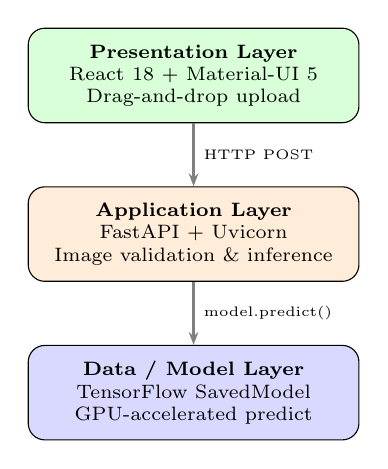
\begin{tikzpicture}[
    node distance=0.8cm,
    tier/.style={rectangle, draw, rounded corners=6pt, minimum width=4.2cm, minimum height=1.2cm, align=center, font=\scriptsize},
    arrow/.style={-{Stealth[scale=0.7]}, thick, color=gray}
]
\node[tier, fill=green!15] (fe) {\textbf{Presentation Layer}\\React 18 + Material-UI 5\\Drag-and-drop upload};
\node[tier, fill=orange!15, below=of fe] (be) {\textbf{Application Layer}\\FastAPI + Uvicorn\\Image validation \& inference};
\node[tier, fill=blue!15, below=of be] (ml) {\textbf{Data / Model Layer}\\TensorFlow SavedModel\\GPU-accelerated predict};

\draw[arrow] (fe) -- node[right, font=\tiny, color=black] {HTTP POST} (be);
\draw[arrow] (be) -- node[right, font=\tiny, color=black] {model.predict()} (ml);
\end{tikzpicture}
\caption{Three-tier web application architecture}
\label{fig:architecture}
\end{figure}

Key implementation details:
\begin{itemize}[noitemsep]
    \item \textbf{Backend (FastAPI):} Asynchronous REST API at \texttt{POST /predict}, accepts multipart image upload with a \texttt{plant\_type} query parameter. Includes CORS middleware, image brightness validation, and a 50\% minimum confidence threshold to reject non-leaf images.
    \item \textbf{Frontend (React 18):} Single-page application with plant-type toggle (Potato/Tomato), drag-and-drop image upload via \texttt{react-dropzone}, color-coded disease results, confidence progress bar, and a prediction history panel (stored in \texttt{localStorage}).
    \item \textbf{Docker Compose:} Single-command deployment (\texttt{docker-compose up}) orchestrating backend ($:$8000) and frontend ($:$3000) containers.
\end{itemize}


% ==========================================================
\section{Experiments and Results}
% ==========================================================

\subsection{Experimental Setup}
\textbf{Hardware:} NVIDIA GeForce RTX 3050 GPU (4\,GB VRAM)\\
\textbf{Software:} Python 3.10, TensorFlow 2.10.1, CUDA 11.2, cuDNN 8.9

\subsection{Results}
Both models were trained for 50 epochs with early convergence observed around epoch 30--35.

\begin{table}[h]
\centering
\caption{Model Performance Summary}
\begin{tabular}{@{}lcccc@{}}
\toprule
\textbf{Model} & \textbf{Train Acc} & \textbf{Val Acc} & \textbf{Test Acc} & \textbf{Classes} \\
\midrule
Potato & 98.2\% & 96.5\% & \textbf{97.2\%} & 3 \\
Tomato & 95.8\% & 92.3\% & \textbf{89.6\%} & 10 \\
\bottomrule
\end{tabular}
\label{tab:results}
\end{table}

\textbf{Key observations:}
\begin{itemize}[noitemsep]
    \item Training curves showed steady convergence with minimal overfitting, validating the augmentation strategy.
    \item Potato's higher accuracy is attributed to its smaller classification space (3 vs.\ 10 classes) and more uniform per-class sample counts.
    \item Tomato's confusable classes (e.g., Early Blight vs.\ Late Blight) account for the lower accuracy.
\end{itemize}


% ==========================================================
\section{Discussion}
% ==========================================================

\subsection{Performance Analysis}
The results are consistent with prior work~\cite{mohanty2016using}. The potato model (97.2\%) matches or exceeds benchmarks reported in the literature for 3-class potato classification. The tomato model (89.6\%) faces greater difficulty due to visual overlap between diseases like Early Blight, Late Blight, and Septoria Leaf Spot, which share similar lesion morphology.

\subsection{Impact of Data Augmentation}
Without augmentation, validation accuracy plateaued at $\sim$80\%. With the five-technique augmentation pipeline, validation accuracy improved by 12--15\%, confirming the importance of augmentation in small-to-medium sized datasets.

\subsection{Image Validation Pipeline}
A practical enhancement not typically found in academic prototypes is the backend's image validation: before running inference, the system checks image brightness (rejects too-dark or overexposed images) and enforces a 50\% confidence threshold. These measures reduce false positives when non-leaf images are submitted.

\subsection{Challenges}
\begin{itemize}[noitemsep]
    \item GPU setup required precise CUDA/cuDNN version matching (CUDA~11.2 + cuDNN~8.9 for TensorFlow~2.10.1)
    \item Class imbalance in the tomato dataset (Mosaic Virus: 373 vs.\ Yellow Leaf Curl: 5,357) affects minority-class recall
    \item PlantVillage images were collected under controlled conditions---real-world field images may exhibit domain shift
\end{itemize}

\subsection{Limitations}
\begin{itemize}[noitemsep]
    \item Coverage limited to potato and tomato crops
    \item No support for multiple simultaneous infections on a single leaf
    \item Model performance degrades on blurry or partially occluded leaf images
    \item No treatment or management recommendations are provided alongside diagnosis
\end{itemize}


% ==========================================================
\section{Conclusion and Future Work}
% ==========================================================

This project successfully delivered \textit{LeafScan AI}, an end-to-end plant disease classification system achieving \textbf{97.2\%} test accuracy on potato and \textbf{89.6\%} on tomato across 13 disease classes. The system is deployed as a full-stack web application with Docker support, demonstrating the practical applicability of deep learning in precision agriculture.

\textbf{Future Work:}
\begin{enumerate}[noitemsep]
    \item Extend coverage to additional crops (wheat, rice, corn)
    \item Adopt transfer learning with pre-trained architectures (ResNet, EfficientNet) for potentially higher accuracy
    \item Develop a mobile application for offline field use
    \item Integrate disease management recommendations alongside diagnosis
    \item Address class imbalance with techniques such as SMOTE or focal loss
\end{enumerate}


% ==========================================================
\section{Artifacts and Acknowledgments}
% ==========================================================

\begin{itemize}[noitemsep]
    \item \textbf{Code Repository:} \url{https://github.com/Ashutosh-yadav0001/Pototo-disease}
    \item \textbf{Dataset:} PlantVillage Dataset~\cite{plantvillage} (Kaggle)
    \item \textbf{Tech Stack:} Python, TensorFlow / Keras, FastAPI, React 18, Docker
\end{itemize}

\textbf{Acknowledgments:} The initial project idea was inspired by the Codebasics YouTube channel~\cite{codebasics2022potato}. AI tools (Antigravity / Gemini) were used to enhance productivity. All work reflects original understanding, implementation, and extension by the author.


% ==========================================================
% References
% ==========================================================
\vfill\pagebreak
{\fontsize{8}{9}\selectfont
\bibliographystyle{IEEEbib}
\bibliography{refs}
}

\end{document}
